\chapter{Gestión}

En este capítulo se detalla la gestión realizada de todos los elementos involucrados en el desarrollo de un proyecto.

\section{Gestión del código y de la documentación}

Por supuesto, una parte fundamental de un proyecto TIC es el código y la documentación. Estos dos elementos son la base de todo el proyecto, por lo que habrá que gestionarlos de forma eficiente y correcta.

Dado que son cruciales, será imprescindible asegurar su seguridad ante pérdidas, ya que son elementos sobre los que se invierte mucho tiempo. Siguiendo el plan de actuación contra el riesgo de perder información del proyecto, se efectuarán backup y controles de versiones de ambos elementos.

En primer lugar, para la gestión del código, en vez de alojar simplemente este código de manera local, lo que suele hacer en la mayoría de los proyectos actuales es crear un repositorio privado, llamado \href{https://github.com/Mario-Carmona/SARA_Chatbot}{SARA\_Chatbot}, en la plataforma GitHub \footnote{\url{https://github.com}}. Una vez tenemos un repositorio privado donde tener un sistema de control de versiones a la vez que sirve de backup, es necesario sincronizar este repositorio que está en la nube, con un repositorio local para poder trabajar con el código. A través de esta sincronización se irán actualizando ambos repositorios conforme se vaya modificando el código y el programador vaya enviando commits. Un commit no es más que una petición para guardar los cambios en el sistema de control de versiones del repositorio privado en GitHub. Para la edición de todo el código se hará uso del editor de código Visual Studio Code.

Y en segundo lugar, para la gestión de la documentación, de igual modo que se hace con el código, se alojará en GitHub, aunque se gestionará de una forma distinta a la realizada con el código. De igual modo, se creará un repositorio privado, llamado \href{https://github.com/Mario-Carmona/Memoria_TFG}{Memoria\_TFG}; y un repositorio local. La diferencia con la gestión del código llega a la hora de la edición de la documentación. Para la edición de la documentación se hará empleo de la plataforma online Overleaf \footnote{\url{https://es.overleaf.com}}, una de las plataformas más empleadas para la edición de documentos escritos en LaTeX. La gestión de la documentación se podría hacer sin necesidad de tener un repositorio local, dado que Overleaf tiene una herramienta para sincronizar los proyectos alojados en Overleaf con repositorios de GitHub. Pero como para efectuar esta sincronización con Overleaf es necesaria una cuenta de pago, y una de las prioridades de este proyecto es minimizar el uso de recursos de pago, para simular esta sincronización se ha creado un repositorio local y además se ha creado un script para la descarga del proyecto completo de la plataforma Overleaf y su posterior movimiento al repositorio local. Además, opcionalmente se puede usar el script para realizar el movimiento del proyecto descargado y un posterior commit al repositorio en Github.

\section{Gestión de recursos} \label{sec:gest_recursos}

\subsection{Recursos humanos}

En la gestión de los recursos humanos se gestiona todo lo relacionado con las personas que trabajan en el proyecto. Dado que este proyecto se efectúa en el marco de un Trabajo de Fin de Grado, la lista de personas involucradas en el proyecto es muy reducida. En concreto, el personal del proyecto es el siguiente:

\begin{itemize}
\item \textbf{Mario Carmona Segovia}, alumno en el grado de Ingeniería Informática en la Escuela Técnica Superior de Ingenierías Informática y Telecomunicación de la Universidad de Granada.
\item \textbf{Dña. Rocío Celeste Romero Zaliz}, profesora del Departamento de Ciencias de la Computación e Inteligencia Artificial de la Universidad de Granada, en calidad de tutora del proyecto.
\end{itemize}

Los roles dentro del proyecto de cada uno de los integrantes del mismo se detalló en el apartado \ref{sec:apli_scrum}. En concreto, el tutor del proyecto era el Product owner, y yo como alumno realizaba el resto de roles del proyecto.

\subsection{Recursos materiales para el desarrollo}

Los recursos materiales utilizados para el desarrollo del proyecto han sido muy pocos. En concreto, se han usado los siguientes recursos:

\begin{itemize}
\item \textbf{Portátil Personal}: Lenovo Legion Y520 con un procesador Intel Core i7-7700HQ, una arquitectura de 64 bits, y una memoria RAM de 16 GB. Con este recurso se elabora toda la programación y la documentación del proyecto.
\item \textbf{\href{https://dasci.es/es/sobre-dasci/recursos/recursos-tecnologicos/}{Servidores GPU del Instituto DaSCI}}: Estos servidores están compuestos por una serie de nodos de cómputo unidos a un nodo cabecera, sobre el cual se hacen las peticiones. Estas peticiones son gestionadas por un gestor de colas, en concreto el gestor es SLURM. Los nodos de cómputo se dividen en varias colas, con la cuenta que se me concedió al poco de iniciar el proyecto, únicamente puedo acceder a los nodos de cómputo situados en la cola \textit{dios}. Dentro de los servidores a cada usuario se le asigna un espacio de almacenamiento donde se puede guardar de forma permanente el código a ejecutar en los servidores.
\end{itemize}

\subsection{Recursos software} \label{subsec:recur_software}

Los recursos software engloban a todas aquellas herramientas software utilizadas para el desarrollo del proyecto. Siguiendo con la filosofía de intentar reducir al máximo los costes, se han usado en su mayoría herramientas de software libre o gratuitas. Las herramientas utilizadas son las siguientes:

\begin{itemize}
\item \textbf{Sistema Operativo}: El S.O. empleado es la distribución de Linux más utilizada en el ámbito personal a nivel mundial, Ubuntu. En concreto, se ha usado la versión Ubuntu 20.04.4 LTS. Este sistema operativo es de software libre.
\item \textbf{GitHub}: Es la plataforma donde se alojará todo el código y la documentación del proyecto. Esta herramienta es una de las plataformas de software libre de alojamiento de código más empleadas a nivel mundial. Además, es usada como gestor de versiones para el proyecto.
\item \textbf{Git}: Es un software de control de versiones. Es el software empleado por GitHub para el control de versiones de su plataforma.
\item \textbf{Visual Studio Code}: Es un editor de código fuente. Con este editor se desarrolla todo el código del proyecto. Este editor es de software libre.
\item \textbf{Heroku}: Es una plataforma que proporciona servicios de computación en la nube. Aunque no es en su totalidad un software libre, para este proyecto he hecho uso de la versión gratuita de la plataforma. El inconveniente de esta versión gratuita es que no se puede utilizar el sistema en producción, solamente para hacer pruebas. Para tener una idea de los distintos planes que existen en Heroku, en la Figura \ref{fig:planes_app_heroku} se muestran todos los planes de pago, y adicionalmente en la Figura \ref{fig:planes_dynos_heroku} se muestran todos los niveles de dynos que existen en Heroku. Un dyno es un contenedor, ya que Heroku divide su potencia de cómputo en unidades, y esas unidades son los dynos. Adicionalmente, es interesante también poder visualizar los planes que existen para añadir una base de datos a la app alojada en Heroku, estos planes para la base de datos se pueden ver en la Figura \ref{fig:planes_postgres_heroku}.

\begin{figure}[H]
\centering
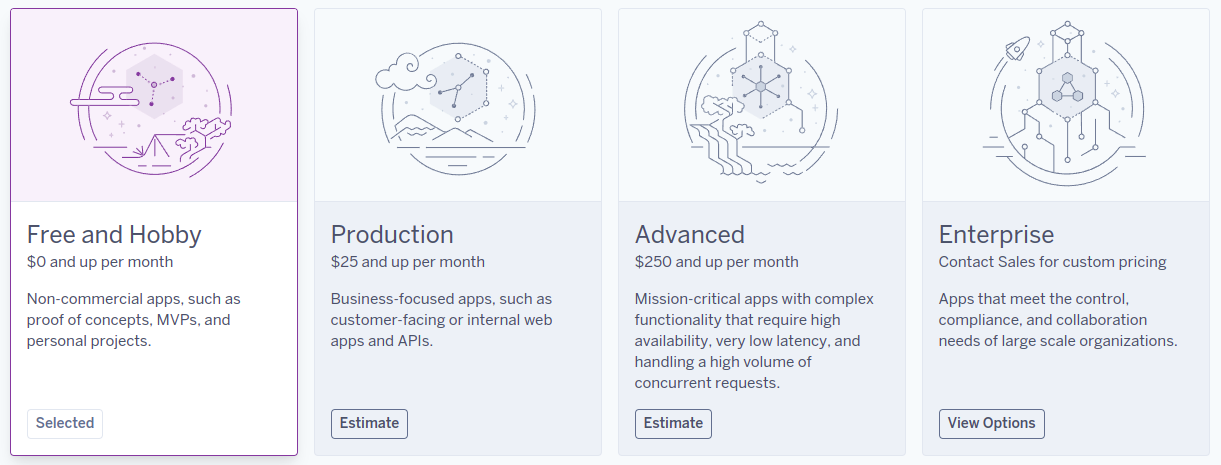
\includegraphics[width=1.0\textwidth]{imagenes/05_Gestion/planes_heroku.png}
\begin{center}
Fuente: \url{https://www.heroku.com/pricing}
\end{center}
\caption{Planes de pago sobre las apps de Heroku}
\label{fig:planes_app_heroku}
\end{figure}

\begin{figure}[H]
\centering
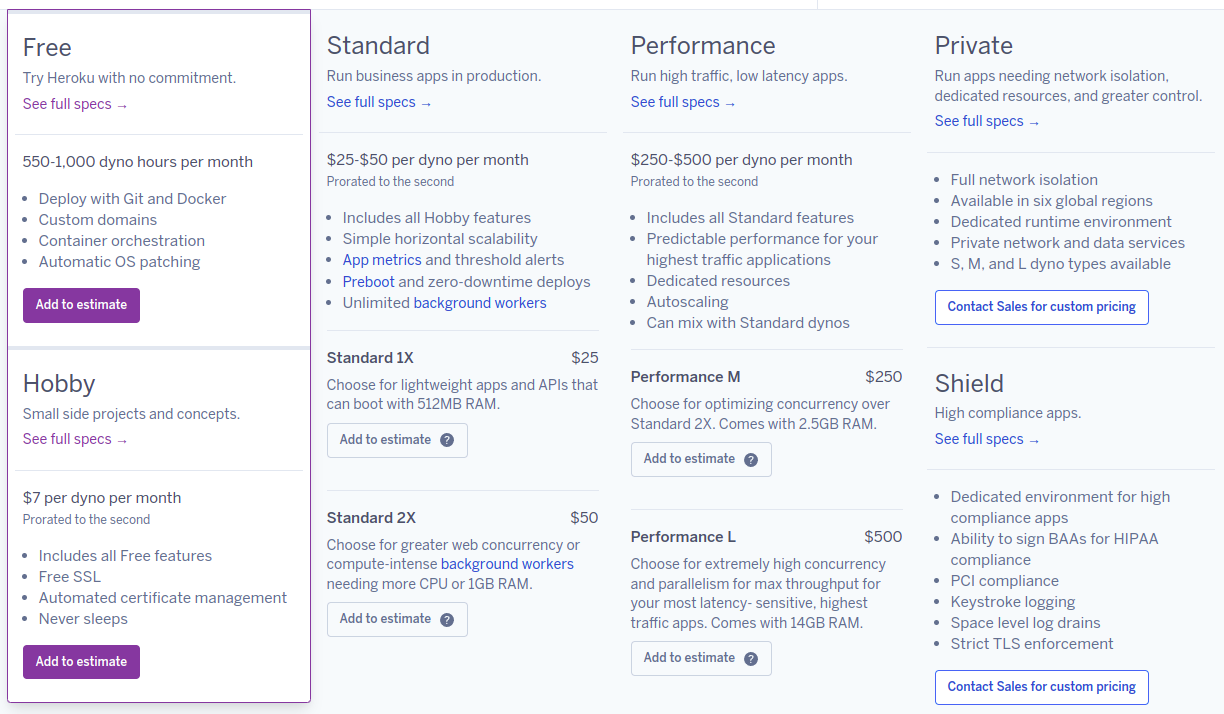
\includegraphics[width=1.0\textwidth]{imagenes/05_Gestion/planes_dynos_heroku.png}
\begin{center}
Fuente: \url{https://www.heroku.com/pricing}
\end{center}
\caption{Planes de pago sobre los dynos de Heroku}
\label{fig:planes_dynos_heroku}
\end{figure}

\begin{figure}[H]
\centering
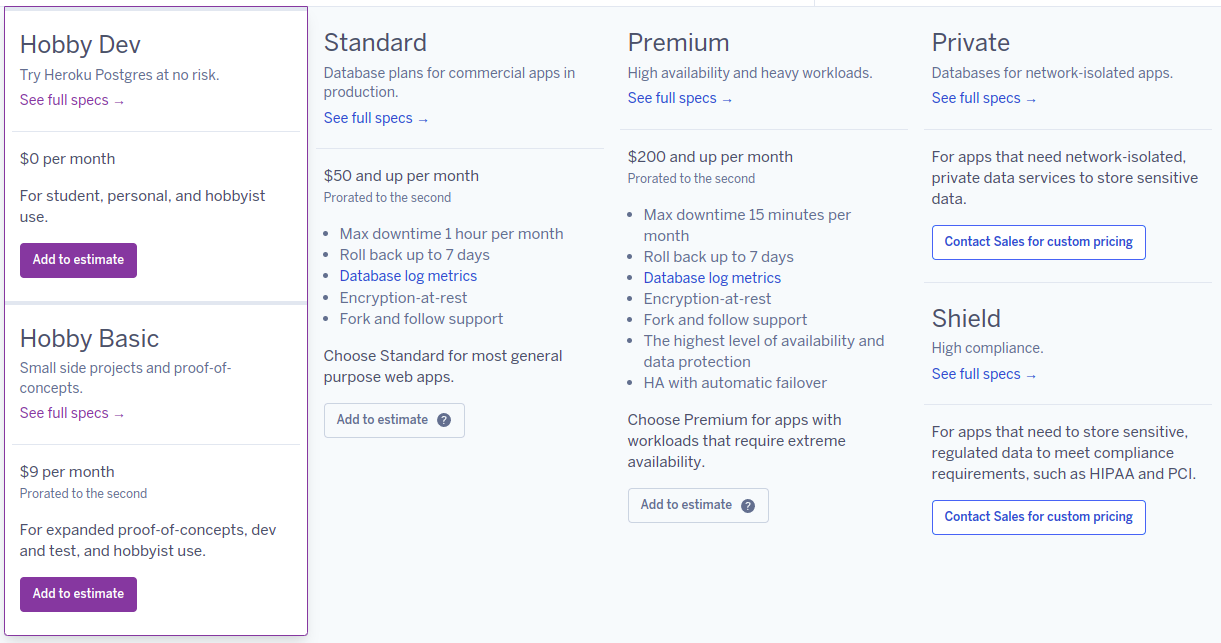
\includegraphics[width=1.0\textwidth]{imagenes/05_Gestion/planes_postgres_heroku.png}
\begin{center}
Fuente: \url{https://www.heroku.com/pricing}
\end{center}
\caption{Planes de pago sobre las bases de datos de Heroku}
\label{fig:planes_postgres_heroku}
\end{figure}

\item \textbf{BlenderBot}: Es una herramienta de software libre para la creación del chatbot.
\item \textbf{Dialogflow}: Es una herramienta para el despliegue del chatbot. Se hará uso de la versión gratuita de la herramienta.
\end{itemize}

\subsection{Recursos de comunicación y documentación} \label{subsec:recur_comu_docu}

Todo buen proyecto debe ser resultado de una buena comunicación entre su personal. Además, se debe elaborar una documentación de calidad para conseguir que el proyecto sea accesible por personas ajenas al desarrollo del proyecto. Para conseguir estos objetivos se ha hecho uso de varias herramientas, entre las cuales se encuentran las siguientes:

\begin{itemize}
\item \textbf{Google Meet}: Es un servicio de videotelefonía desarrollado por Google. Este servicio se ha utilizado para realizar las distintas reuniones con el tutor.
\item \textbf{Correo UGR}: Es un servicio de correo electrónico de la UGR. Este servicio se ha utilizado para realizar conversaciones con el tutor sobre temas puntuales o de menor peso.
\item \textbf{Overleaf}: Es una plataforma de edición de documentos escritos en LaTeX. Esta plataforma se ha usado para la elaboración de la documentación del proyecto.
\item \textbf{Texmaker}: Es un editor empleado para desarrollar documentos con LaTeX.
\item \textbf{Visual Paradigm}: Es una herramienta de modelado de diagramas de desarrollo software. En principio es una herramienta de pago, pero la UGR dispone de licencias de uso educativo para los estudiantes.
\item \textbf{Microsoft Powerpoint}: Es un programa de presentación desarrollado por Microsoft. Con este programa se ha elaborado la presentación del proyecto.
\end{itemize}



\section{Gestión de costes}

Todo proyecto debe tener su gestión de costes para evaluar la viabilidad económica del proyecto. En la gestión de costes se tiene en cuenta el coste derivado de cada uno de los recursos citados en el apartado \ref{sec:gest_recursos}.

\subsection{Costes de recursos humanos}

Los costes de recursos humanos vienen derivados del trabajo realizado por el equipo de desarrollo, como en este proyecto este equipo está formado por una única persona, el alumno, el coste de recursos humanos será el equivalente al trabajo realizado por un ingeniero informático durante el desarrollo del proyecto, es decir, se simula que el alumno se trata de un ingeniero informático que trabaja de forma autónoma.

Para estimar este coste de recursos humanos es necesario estimar el coste de ese trabajo y para ello es necesario recabar información.

En primer lugar, es necesario calcular el tiempo que ha estado trabajando el ingeniero. Dado que el proyecto tiene una duración de 5 meses.

\begin{center}
$Dias\ totales\ =\ 5\ meses\ *\ 30\ dias / mes\ =\ 150\ dias$
\end{center}

El tiempo total aproximado será de 150 días. A este tiempo total habrá que descontar los días no laborables. Los días no laborables en estos 5 meses serían aproximadamente:

\begin{center}
$Dias\ no\ laborables\ =\ 5\ meses\ *\ 8\ dias/mes\ =\ 40\ dias$
\end{center}

Por lo tanto, los días laborables gastados por el trabajador son:

\begin{center}
$Dias\ laborables\ =\ Dias\ totales\ -\ Dias\ no\ laborables\ =\ 110\ dias$
\end{center}

Además, dentro de cada día laborable hay una jornada laboral. Normalmente, esta jornada es de 8 horas, pero como el desarrollo del proyecto se ha hecho en conjunto con la realización de otras asignaturas, no se ha dispuesto de todo el tiempo, por lo tanto, se estimará que aproximadamente se ha trabajado unas 5 horas al día. En consecuencia, el número total de horas trabajadas es el siguiente:

\begin{center}
$Horas\ laborables\ =\ Dias\ laborables\ *\ 5\ horas/dia\ =\ 550\ horas$
\end{center}

Este número de horas excede en gran medida el número de horas correspondientes a los ECTS de un TFG. El número mínimo de horas que se debe emplear en el desarrollo de un TFG deben ser 300 horas.

Una vez tenemos el tiempo trabajado por el ingeniero, es necesario obtener que salario tiene este trabajador a la hora. Para obtener esta información me he basado en el estudio de la página talent.com \footnote{\url{https://acortar.link/MiqarT}}. En este estudio se analiza el sueldo medio de un ingeniero informático en España, el salario medio es de 2.208 \EURtm al mes. Por lo tanto, el salario medio por hora será de 13,59 \EURtm.

Con la información recabada ya podemos estimar el coste del trabajo realizado por el ingeniero. El coste total se puede ver en la Tabla \ref{tab:coste_recur_humanos}.

\begin{table}[h]
\centering
\resizebox{\textwidth}{!}{%
\begin{tabular}{@{}cccc@{}}
\toprule
\textbf{Recurso} & \textbf{Precio / Hora}             & \textbf{Nº Horas}    & \textbf{Importe}              \\ \midrule
Trabajo autónomo  & 13,59 \EURtm / hora & 550                  & 7474,50 \EURtm \\ \midrule
\textbf{Total:}   & \multicolumn{1}{l}{}               & \multicolumn{1}{l}{} & 7474,50 \EURtm \\ \bottomrule
\end{tabular}%
}
\caption{Costes asociados a los recursos humanos}
\label{tab:coste_recur_humanos}
\end{table}

\subsection{Costes de recursos materiales}

Los costes derivados de los recursos materiales se calculan de una forma distinta a la realizada en los costes de recursos humanos, por la simple razón de que los recursos materiales se van devaluando con el paso del tiempo tras su adquisición. Por esta razón deberemos calcular el coste de los distintos recursos materiales con la depreciación aplicada.

Para calcular el coste actual del recurso se debe obtener previamente la siguiente información:

\begin{itemize}
\item Coste de adquisición del producto
\item Coste residual del producto, es decir, el valor del producto al final de su vida útil
\item Coeficiente de amortiguación lineal
\end{itemize}

Nos vamos a centrar en el portátil personal, ya que a pesar de que los servidores GPU del Instituto DaSCI tienen un coste de uso, al ser estudiantes de la UGR el coste para nuestro proyecto ha sido nulo y de esta forma lo hemos indicado en el cálculo de los costes; y en el caso de usar servidores en la nube ajenos a la UGR, el coste de estos servidores suele tener un coste fijo cada mes a través de una cuota mensual o en ocasiones el coste de estos servidores se calcula según el tiempo de uso que se haya hecho de estos servidores.

El coste de adquisición del producto es de 1100 \EURtm. Como coste residual fijamos la cantidad de 100 \EURtm. Y por último queda fijar el coeficiente de amortiguación lineal, para fijar este valor he recabado información sobre el coeficiente de amortiguación lineal de los equipos electrónicos. Esta información la encontré en un artículo de la página web Iberley \footnote{\url{https://www.iberley.es/temas/tablas-amortizacion-i-sociedades-30681}}, donde se indica que el coeficiente de amortiguación lineal máximo para estos equipos electrónicos es del 20\%.

Para calcular el coste actual del producto se utiliza la siguiente fórmula:

\begin{center}
$C_{ac}\ =\ (C_{ad}\ -\ C_{re})\ *\ C_{amor}$\\
$C_{ac}:\ Coste\ actual$\\
$C_{ad}:\ Coste\ adquisicion$\\
$C_{re}:\ Coste\ residual$\\
$C_{amor}:\ Coeficiente\ amortiguacion$
\end{center}

Siguiendo esta fórmula, el coste actual del portátil es de 200 \EURtm. Pero este coste indica el coste anual del recurso, por lo que habrá que calcular el coste del recurso teniendo en cuenta el tiempo de empleo. El tiempo de uso es el mismo que el tiempo trabajado por el alumno, es decir, 5 meses trabajando los 5 días laborables de la semana a razón de 5 horas por día. Basándonos en los cálculos del anterior apartado, el total de horas laborables es de 550 horas. Por lo que el coste final del portátil es el siguiente:

\begin{center}
$Coste\ final\ =\ 200\ *\ \frac{550}{1200}\ =\ 91,66\ euros$
\end{center}

Al igual que se hace con los costes asociados a los recursos humanos, en este caso se puede ver un resumen de los costes asociados a los recursos materiales en la Tabla \ref{tab:coste_recur_materiales}.

\begin{table}[h]
\centering
\resizebox{\textwidth}{!}{%
\begin{tabular}{@{}cccc@{}}
\toprule
\textbf{Recurso}  & \textbf{Precio / Hora}            & \textbf{Nº Horas}    & \textbf{Importe}            \\ \midrule
Portátil personal & 0,16 \EURtm / hora & 550                  & 91,66 \EURtm \\ \midrule
\textbf{Total:}   & \multicolumn{1}{l}{}              & \multicolumn{1}{l}{} & 91,66 \EURtm \\ \bottomrule
\end{tabular}%
}
\caption{Costes asociados a los recursos materiales}
\label{tab:coste_recur_materiales}
\end{table}

\subsection{Costes de recursos software}

En este apartado se estima el coste de todos los recursos software listados en el apartado \ref{subsec:recur_software}. Tal y como se indica en este apartado, todos los recursos software utilizados son de software libre, y en concreto con Heroku, aunque no es un software gratuito, sí que dispone de una versión gratuita que tiene ciertas limitaciones, pero que nos sirve para el desarrollo del proyecto.

\subsection{Costes de recursos de comunicación y documentación}

En este apartado se estima el coste de todos los recursos para la comunicación con la tutora y la elaboración de la documentación. Al igual que pasa con el apartado anterior, tal y como se indica en el apartado \ref{subsec:recur_comu_docu}, todos los recursos empleados son de software libre, aunque hace falta puntualizar que la herramienta Visual Paradigm es de pago, pero como la UGR dispone de licencias gratuitas para los alumnos, se ha aprovechado esta ventaja para la elaboración de los diagramas del diseño del proyecto.

\subsection{Costes adicionales}

Dentro de los costes adicionales se tiene el coste derivado de todos aquellos recursos que no hayan sido listados en ninguno de los anteriores apartados. Los principales recursos de este apartado son el Internet y la factura de la luz. La tarifa de Internet contratada tiene un coste de 30 \EURtm/mes, por lo tanto, el coste total por el Internet asciende a 150 \EURtm. Y en cuanto a la factura de la luz, es un coste más difícil de calcular, dado que hay muchas variables que intervienen en su valor, pero una posible estimación sobre su valor podría ser 25 \EURtm. El coste total derivado de estos recursos adicionales se puede ver en la Tabla \ref{tab:coste_recur_adicionales}.

\begin{table}[h]
\centering
\resizebox{0.5\textwidth}{!}{%
\begin{tabular}{@{}cc@{}}
\toprule
\textbf{Recurso}  & \textbf{Importe}             \\ \midrule
Internet          & 150,00 \EURtm \\ \midrule
Factura de la luz & 25,00 \EURtm  \\ \midrule
\textbf{Total:}   & 175,00 \EURtm \\ \bottomrule
\end{tabular}%
}
\caption{Costes asociados a los recursos adicionales}
\label{tab:coste_recur_adicionales}
\end{table}



\section{Presupuesto total}

Para tener una visión global de todos los costes analizados se ha elaborado una tabla donde se desglosa toda la información de cada apartado y finalmente se calcula el coste acumulado de todo el proyecto. Estos datos se pueden ver en la Tabla \ref{tab:presupuesto_total}.


\begin{longtable}[c]{@{}lr@{}}
\toprule
\textbf{Recurso}                     & \textbf{Importe}                       \\
\endhead
%
\bottomrule
\endfoot
%
\endlastfoot
%
                                     &                                        \\* \midrule
\textbf{Costes de recursos humanos}  & \textbf{7474,50 \EURtm} \\
                                     & \multicolumn{1}{l}{}                   \\
Trabajo autónomo                     & 7474,50 \EURtm          \\* \midrule
\textbf{Costes de recursos materiales}                      & \textbf{91,66 \EURtm} \\
                                     & \multicolumn{1}{l}{}                   \\
Portátil personal                    & 91,66 \EURtm            \\
Servidores GPU del Instituto DaSCI             & 0,00 \EURtm             \\* \midrule
\textbf{Costes de recursos software} & \textbf{0,00 \EURtm}    \\
                                     & \multicolumn{1}{l}{}                   \\
Sistema Operativo                    & 0,00 \EURtm             \\
GitHub                               & 0,00 \EURtm             \\
Git                                  & 0,00 \EURtm             \\
Visual Studio Code                   & 0,00 \EURtm             \\
Heroku                               & 0,00 \EURtm             \\
BlenderBot                           & 0,00 \EURtm             \\
Dialogflow                           & 0,00 \EURtm             \\* \midrule
\textbf{Costes de recursos de comunicación y documentación} & \textbf{0,00 \EURtm}  \\
                                     & \multicolumn{1}{l}{}                   \\
Google Meet                          & 0,00 \EURtm             \\
Correo UGR                           & 0,00 \EURtm             \\
Overleaf                             & 0,00 \EURtm             \\
Texmaker                             & 0,00 \EURtm             \\
Visual Paradigm                      & 0,00 \EURtm             \\
Microsoft Powerpoint                 & 0,00 \EURtm             \\* \midrule
\textbf{Costes adicionales}          & \textbf{175,00 \EURtm}  \\
                                     & \multicolumn{1}{l}{}                   \\
Internet                             & 150,00 \EURtm           \\
Factura de la luz                    & 25,00 \EURtm            \\
                                     & \multicolumn{1}{l}{}                   \\* \midrule
\multicolumn{1}{r}{\textbf{Total:}}  & \textbf{7741,16 \EURtm} \\* \bottomrule
\caption{Presupuesto total del proyecto}
\label{tab:presupuesto_total}
\end{longtable}
























